% The Navier-Stokes workbench: the exact radius of the Rindler shear series, and curvature rates for the map to Yang-Mills.
% Prepared by Claude (Anthropic), model claude-opus-5-5 (Opus 5.5).
% Compile with lualatex (three times).
% The Navier-Stokes workbench: the exact radius of the Rindler shear series, and curvature rates for the map to Yang-Mills.
% Prepared by Claude (Anthropic), model claude-opus-5-5 (Opus 5.5).
% Compile with lualatex (three times).
\documentclass[11pt,a4paper]{article}
\usepackage[a4paper,margin=24mm,headheight=14pt]{geometry}
\usepackage{fontspec}
\directlua{luaotfload.add_fallback("readerfallback",{"TeX Gyre Pagella Math:mode=harf;","STIX:mode=harf;","DejaVu Serif:mode=harf;","FreeSerif:mode=harf;"})}
\setmainfont{TeX Gyre Pagella}[RawFeature={fallback=readerfallback}]
\setsansfont{TeX Gyre Heros}[Scale=MatchLowercase]
\setmonofont{DejaVu Sans Mono}[Scale=0.84]
\usepackage{amsmath,amsthm,mathtools}
\usepackage{graphicx}
\graphicspath{{fig/}}
\usepackage{unicode-math}
\setmathfont{TeX Gyre Pagella Math}
\usepackage{microtype}
\usepackage{booktabs,longtable,array,tabularx}
\usepackage{enumitem}
\setlist{itemsep=2pt,topsep=4pt,leftmargin=*}
\usepackage[dvipsnames]{xcolor}
\usepackage{fancyhdr}
\usepackage{titlesec}
\usepackage[hidelinks,bookmarksnumbered]{hyperref}
\hypersetup{pdftitle={The Navier-Stokes workbench: the exact radius of the Rindler shear series, and curvature rates for the map to Yang-Mills},
  pdfauthor={Claude (Anthropic), model claude-opus-5-5; workbench by KokunoYumeto},
  pdfsubject={Paper on the Navier-Stokes workbench of KokunoYumeto},
  pdfkeywords={Navier-Stokes, finite-time blowup, Rindler fluid, fluid/gravity, hydrodynamic series, radius of convergence, pole collision, Krawczyk, Yang-Mills}}
\usepackage{bookmark}

\titleformat{\section}{\normalfont\Large\bfseries}{\thesection}{0.8em}{}
\titleformat{\subsection}{\normalfont\large\bfseries}{\thesubsection}{0.7em}{}
\titlespacing*{\section}{0pt}{2.2ex plus 1ex}{1.2ex}
\titlespacing*{\subsection}{0pt}{1.8ex plus .8ex}{0.9ex}

\pagestyle{fancy}
\fancyhf{}
\fancyhead[L]{\small\itshape The Navier--Stokes workbench}
\fancyhead[R]{\small\thepage}
\renewcommand{\headrulewidth}{0.3pt}
\fancypagestyle{plain}{\fancyhf{}\fancyfoot[C]{\small\thepage}\renewcommand{\headrulewidth}{0pt}}

\theoremstyle{plain}
\newtheorem{theorem}{Theorem}[section]
\newtheorem{proposition}[theorem]{Proposition}
\newtheorem{lemma}[theorem]{Lemma}
\newtheorem{corollary}[theorem]{Corollary}
\newtheorem{introthm}{Theorem}
\renewcommand{\theintrothm}{\Roman{introthm}}
\theoremstyle{definition}
\newtheorem{definition}[theorem]{Definition}
\newtheorem{example}[theorem]{Example}
\theoremstyle{remark}
\newtheorem{remark}[theorem]{Remark}

% status line printed under a statement
\newcommand{\status}[1]{\par\smallskip\noindent{\small\color{black!70}\textsf{Status.}\ #1}\par\smallskip}
\newcommand{\negres}[2]{\par\smallskip\noindent\textbf{#1}\ #2\par}

% notation
\newcommand{\B}{\mathcal{B}}
\newcommand{\Zs}{\mathcal{Z}}
\newcommand{\C}{\mathbb{C}}
\newcommand{\R}{\mathbb{R}}
\newcommand{\Q}{\mathbb{Q}}
\newcommand{\ZZ}{\mathbb{Z}}
\newcommand{\NN}{\mathbb{N}}
\newcommand{\Ff}{\mathbb{F}}
\newcommand{\re}{\operatorname{Re}}
\newcommand{\im}{\operatorname{Im}}
\newcommand{\Res}{\operatorname*{Res}}
\newcommand{\sgn}{\operatorname{sgn}}
\newcommand{\Gr}{\operatorname{Gr}}
\newcommand{\cl}{\overline}
\newcommand{\note}[1]{\texttt{#1}}
\newcommand{\lbl}[1]{\textsf{#1}}

\setlength{\parskip}{3pt}
\setlength{\emergencystretch}{2.5em}
\setlength{\parindent}{0pt}

\newcommand{\T}{\mathcal{T}}
\newcommand{\Hs}{\mathcal{H}}
\newcommand{\lcm}{\operatorname{lcm}}
\newcommand{\TV}{\operatorname{TV}}
\newcommand{\tr}{\operatorname{tr}}
\newcommand{\Var}{\operatorname{Var}}


\begin{document}
\thispagestyle{plain}
\begin{center}
{\LARGE\bfseries The Navier--Stokes workbench}\\[8pt]
{\Large The exact radius of the Rindler shear series,\\ and curvature rates for the map to Yang--Mills}\\[14pt]
{\large A paper prepared from an audit of the workbench by Claude (Anthropic),\\ model \texttt{claude-opus-5-5}}\\[8pt]
{\normalsize Workbench: KokunoYumeto (\texttt{KokunoYumeto/yang-mills-interacting-workbench}, folder \texttt{navier-stokes/});\\ imported construction: OpenAI, \emph{Finite Time Blowup for Navier--Stokes}}\\[4pt]
{\normalsize Audit 27 September 2026; 27 September 2026 (the typeset version of the audit note \texttt{51\_} and of its condensed record; Appendix~\ref{app:changes})}\\[4pt]
{\small Published at the author's request ahead of the author's review; the author may revise or withdraw it.}\\[2pt]
{\small Companion to the paper on the Yang--Mills workbench, in the Zenodo record 10.5281/zenodo.22883643 and its later versions}
\end{center}

\begin{abstract}
\noindent
OpenAI's manuscript \emph{Finite Time Blowup for Navier--Stokes} constructs, for every viscosity, a smooth solution of the forced three-dimensional Navier--Stokes equations with bounded energy that blows up in finite time. A workbench built by KokunoYumeto with AI systems reconstructs the construction, continues it into a vacuum-hydrodynamics model, and connects it to Yang--Mills and other programmes. This paper states what the workbench establishes and proves three kinds of results.

First, for the shear sector of the cutoff Rindler fluid of the continuation, the hydrodynamic dispersion series $\omega(k)=-i\nu k^2-i(3\nu^3/2c^2)k^4-\cdots$ has radius of convergence exactly $k_*=0.389236400495165\ldots\,c/\nu$. The radius is set by a certified collision of the diffusive pole with the first non-hydrodynamic pole at purely imaginary frequency; the mode is purely damped up to it, the coefficients have exact square-root asymptotics, and the series summed on its circle of convergence returns the collision frequency. These statements are proved with computer assistance in ball arithmetic and verified independently with a second interval library. Second, conditionally on four named statements of the manuscript, the curvature masses of the workbench's map from Navier--Stokes to Yang--Mills grow at explicit rates. Third, under the same statements the blowup is of Type II, with $\|u\|_{L^3}\gtrsim\tau^{-4h/3}$, and every rate is compared with the classical necessary conditions for a singularity. The manuscript's main theorem is imported and is not verified here.
\end{abstract}

\section*{Introduction}\phantomsection\label{sec:about}
\addcontentsline{toc}{section}{Introduction}

\subsection*{The problem and this record}

OpenAI's manuscript \cite{OpenAINS} is a 166-page construction of finite-time blowup for the forced Navier--Stokes equations in three dimensions. The workbench around it transcribes the manuscript, adds a 208-page reader and programs that replay its identities, and continues it in two directions: into a vacuum-hydrodynamics model built on the cutoff Rindler fluid of fluid/gravity duality, and into typed maps to the author's other programmes, among them Yang--Mills. Two questions about this material are of independent interest and can be settled by computation: whether the hydrodynamic expansion of the continuation's Rindler fluid converges, and how the manuscript's profile estimates translate into rates for the quantities that the map to Yang--Mills uses. This paper settles the first unconditionally and the second conditionally, re-runs every identity of the workbench's first-pass scripts, and states what each map carries.

The workbench is research carried out with AI systems, which its author used to formulate and test many hypotheses quickly. Some of its directions are finished computations, some are programmes with proved parts, and some are proposals; not every direction is expected to hold. An unfinished programme is still mathematics, and its proved parts stand on their proofs whatever becomes of the rest. The audit behind this paper had limited compute and did not examine every direction; where the paper gives a view rather than a proof, the view is labelled as mine and its reasons are given.

\subsection*{Main results}

The continuation's cutoff Rindler fluid has, for shear perturbations $\propto e^{-i\omega t+ikz}$, the dispersion relation $I'_\alpha(q)=0$ with $q=k\rho_c$, $\alpha=-i\omega\rho_c/c$ and $\rho_c=2\nu/c$ (Section~\ref{sec:rindler}). The hydrodynamic root $\alpha_h$ is the zero that tends to $0$ as $q\to0$; in $x=q^2/4$ it has the expansion $\alpha_h(x)=-2x-3x^2-\tfrac{29}3x^3-\cdots$.

\begin{introthm}[Theorems~\ref{thm:collision} and~\ref{thm:radius}]
The function $(\alpha,q)\mapsto I'_\alpha(q)$ has a nondegenerate double zero in $\alpha$ at $(\alpha_*,q_*)$ with $q_*=0.778472800990330076180356446189\pm10^{-20}$ and $\alpha_*=-0.5697140809723617\ldots$. The hydrodynamic root $\alpha_h$ is analytic on the disk $|x|<x_*=q_*^2/4$, real and negative on $0<x<x_*$, and has a square-root branch point at $x_*$. So its Taylor series has radius of convergence exactly $x_*$; in physical units, $\omega(k)$ has radius exactly $k_*=q_*c/(2\nu)=0.389236400495165038\ldots\,c/\nu$, and its first singularity is $\omega_*=-0.2848570405\ldots\,i\,c^2/\nu$.
\end{introthm}

\begin{introthm}[Corollary~\ref{cor:darboux}]
Write $\alpha_h(x)=\sum_{k\ge1}a_kx^k$. Then $a_k=-C\,x_*^{-k}k^{-3/2}\bigl(1+O(1/k)\bigr)$ with a certified constant $C\in[0.14696,0.14757]$. The series converges absolutely on $|x|=x_*$, and $\sum_ka_kx_*^k=\alpha_*$: the dispersion series summed at $k=k_*$ returns the collision frequency.
\end{introthm}

The Yang--Mills repository maps a velocity field $u$ to the abelian connection $A_i=\lambda u_iT$ and uses the curvature masses $\mathcal K_B=\lambda^2\|\operatorname{curl}u\|^2$ and $\mathcal K_E=\lambda^2c^{-2}\|\partial_tu\|^2$. With $\tau=1-t$ and the manuscript's small parameter $0<h<1/100$:

\begin{introthm}[Theorem~\ref{thm:rates}, Proposition~\ref{prop:typeII}]
Conditionally on four named statements (H1)--(H4) of the manuscript, for every viscosity $\nu>0$ and all small $\tau$:
$\|\operatorname{curl}u_\nu(1-\tau)\|_2^2\ge\nu^{3/2}C_\Omega\,\tau^{-1/2-3h}$ and $\|\partial_tu_\nu(1-\tau)\|_2^2\ge\nu^{5/2}C_{\dot u}\,\tau^{-3/2-3h}$; so $\mathcal K_B\to\infty$ with finite integral and $\mathcal K_E\to\infty$ with infinite integral. Moreover $\|u(1-\tau)\|_{L^3}\ge c\,\tau^{-4h/3}$, $\|\omega(1-\tau)\|_\infty\ge c\,\tau^{-1-h}$ and $\tau^{1/2}\|u(1-\tau)\|_\infty\ge c\,\tau^{-h}$: the blowup is of Type~II.
\end{introthm}

\subsection*{What the results mean}

The radius theorem places the breakdown of the hydrodynamic gradient expansion of the Rindler fluid at a specific, certified event: the diffusive mode meets the first non-hydrodynamic mode at purely imaginary frequency and real momentum (Figure~\ref{fig:collision}). This is the flat-cutoff instance of the convergence criterion of Grozdanov, Kovtun, Starinets and Tadić \cite{GKST}, with $\eta/s=1/(4\pi)$, and the partner mode starts at the first Matsubara frequency of the cutoff's Unruh temperature. The conditional rates say how singular the manuscript's solutions are: the blowup exceeds the Type~I rate by the angular Reynolds number $\tau^{-h}$, and the classical necessary conditions for a singularity recalled in Section~\ref{sec:rates} hold with margins that are positive powers of $\tau^{-h}$. For the map to Yang--Mills, the rates are exactly those the repository uses, and their status is conditional on named statements rather than unchecked.

\subsection*{The bridges}

The workbench connects the Navier--Stokes construction to the author's other programmes through explicit maps: an abelian and a non-abelian map to Yang--Mills, the auxiliary torus operator that the Erdős--Straus supplement uses, Mellin transforms toward the zeta programme, a Beltrami solution from the $S^6$ oscillator, the divergence-free field of the Jacobian-conjecture counterexample, and the snapshot and Rindler maps to Einstein gravity. Section~\ref{sec:bridges} states what each carries and what is established about it, with my assessment. In the author's view such connections are among the most valuable outcomes of the research. In my assessment the map to Einstein gravity has produced the strongest result so far, the exact radius of Theorem~I, because it settles a question the continuation left open and is of independent interest in fluid/gravity duality.

\subsection*{How this record was made}

This record is an audit, carried out on 27 September 2026, of the workbench folder \texttt{navier-stokes/} of \texttt{KokunoYumeto/yang-mills-interacting-workbench} at commit \texttt{fa79faf}: the source-faithful transcription of the manuscript (cited \emph{src p.~$N$}), the 208-page workbench reader, and the continuation \texttt{continuations/20260919-vacuum-hydrodynamics/} (cited \emph{RESEARCH.md}). The official PDF of the manuscript was checked against the hash that the transcription freezes (Appendix~\ref{app:verification}). The construction is OpenAI's; the reconstruction, the continuation and the maps are the workbench's, whose author is KokunoYumeto.

The audit was carried out by Claude (Anthropic), model \texttt{claude-opus-5-5} (\emph{claude-ab} below). A first-pass inventory was made by a separate Claude instance, and an independent referee, which wrote none of the text, re-verified the certificate of Theorem~\ref{thm:radius} with a second interval library and read the rest in both directions; its findings were verified by claude-ab before they were applied (Appendix~\ref{app:verification}).

Every statement has one of four statuses: \emph{verified} (proved here, with computer assistance where stated, or re-computed by a program listed in Appendix~\ref{app:verification}); \emph{not verified here}, which implies nothing in either direction; \emph{my assessment}, a view in the first person with its reasons; and \emph{proved negative}, stated with its counterexample or derivation (Section~\ref{sec:negative}). Results that rest on statements of the manuscript are labelled \textsf{Conditional} and name them; they are verified relative to those statements. The manuscript's main theorem is \emph{not verified here}.

The audit note \texttt{51\_} on which this paper is based was withdrawn from the branch \texttt{claude/claude-ab-grind-20260925} on 27 September 2026 because of its framing, together with the other notes. It remains, unchanged, in the branch's history at commit \texttt{a90d9e5b}. The scripts cited here are republished in \texttt{contrib/claude-ab/rewrite/checks/ns/} on the same branch.

\subsection*{Organization}

Section~\ref{sec:setting} states the manuscript's theorem, the architecture of its proof and what the re-run of the workbench's scripts verifies. Section~\ref{sec:rindler} proves the collision, the exact radius and the coefficient asymptotics. Section~\ref{sec:rates} proves the conditional curvature rates and the Type~II classification. Section~\ref{sec:negative} collects the proved limits, Section~\ref{sec:bridges} the typed maps to the other programmes with my assessment, and Section~\ref{sec:open} the questions and what was not checked. Appendix~\ref{app:verification} lists the programs, and Appendix~\ref{app:changes} what this typeset version changes relative to the audit note.


\tableofcontents
\clearpage

\section{The manuscript, the workbench, and what the re-run verifies}\label{sec:setting}

\subsection{The imported theorem}

The manuscript's main theorem, which we call NS-00 as the workbench does, is the following \cite[Theorem~1.1]{OpenAINS}.

\begin{theorem}[NS-00; the manuscript's Theorem~1.1]\label{thm:ns00}
For every $\nu>0$ there are a force $f\in C_c^\infty(\R^3\times(0,\infty))$, a compact set $K$ and a smooth solution $(u,p)$ of the forced Navier--Stokes equations on $\R^3\times[0,1)$ with $u(\cdot,0)=0$, supports in $K$ and $\sup_t\|u(t)\|_2<\infty$, such that $\limsup_{t\uparrow1}\|u(t)\|_\infty=\infty$.
\end{theorem}
\status{Imported; \emph{not verified here}. Corollary~10.6 of the manuscript (src p.~125) is the periodic version. The workbench is a reconstruction and verification reader of this theorem, and its own ledger lists four items as unfinished.}

\subsection{The architecture of the proof}

The workbench's reader follows the manuscript's architecture, which we recall for orientation; none of these steps is verified here.
\begin{itemize}
\item \emph{Force as residual} (src p.~3). For any incompressible $(u,p)$ put $f:=\partial_tu+(u\cdot\nabla)u-\nu\Delta u+\nabla p$. The work is to make $f$ smooth through $t=1$ while $\|u\|_\infty\to\infty$.
\item \emph{A slender core} (src p.~4). It has radial scale $\ell_r\asymp\tau^{1/2}$, axial scale $\ell_z\asymp\tau^{1/2-h}$ and speed $|u_\theta|,|u_z|\asymp\tau^{-1/2-h}$, with $\tau=1-t$ and $0<h<1/100$. The core energy is $\asymp\tau^{1/2-3h}$ and the angular Reynolds number is $\mathrm{Re}_\theta\asymp\tau^{-h}$. The similarity coordinates are (src (3.2))
\[
\tau=q(1-\eta^2),\qquad z=q^D\eta,\qquad r^2=2qX,\qquad A=\tfrac12+h,\qquad D=\tfrac12-h.
\]
\item \emph{Profiles} (Theorem~4.6, src p.~32). The tangential residuals are exact radial divergences of a stress $q^{-A-1/2}T_0$, with $T_0=0$ on the inner region $X\le X_a$ and admissible on the annulus; the exterior is an exact heat solution.
\item \emph{Base correction} (Proposition~5.5, src p.~60). The residual of the base field equals stress divergences plus a flat remainder. The profile estimates (5.42) hold uniformly on $[X_{\mathrm{lo}},X_{\mathrm{hi}}]\times[-1,1]$ for the summed background, with the Stokes streamfunctions summed before differentiation.
\item \emph{Waves and corrections} (§§6--9). Pulses on an auxiliary torus with the matrix $J=\begin{psmallmatrix}3&1\\1&5\end{psmallmatrix}$ realise the stress through their covariance (Proposition~7.5); a four-step cycle raises the residual exponent $\sigma_j=\frac15+\frac j{10}\to\infty$; a summation with shrinking cutoffs (Proposition~9.9) gives the manuscript's Theorem~3.1.
\item \emph{The endpoint} (§10). Potential-first cutoffs (Proposition~10.1) are used; the force jets converge (Lemma~10.2) and are extended by a Borel series past $t=1$ (Lemma~10.3); energy and uniqueness follow (Lemmas~10.4--10.5). The growth path is (10.20)--(10.21), the viscosity map is (10.22), and the periodisation is Corollary~10.6.
\end{itemize}

\subsection{What the re-run of the workbench's scripts verifies}

The first-pass inventory classified the manuscript's statements and the thirteen reconstruction components of the workbench. Its ten scripts were re-run here with python-flint 0.9.0, sympy 1.14.0 and mpmath 1.3.0, and their outputs agree with the shipped ones line for line, apart from timing lines. They comprise $251$ identity checks and the $5$ conditions of the collision certificate, all passing, and $4$ negative controls, all correctly rejected. The workbench's own replay, of $9$ programs and $144$ result groups, passes as well.

The identities verified in this way are:
\begin{itemize}
\item the leading-field calculus, including $R^{(0)}=-(\partial_r+k/r)(q^{-A-1/2}T_0)$ in full;
\item the order-$n$ coefficient equations for $n\le2$, from the full residual;
\item the actual-shear correction (AS7)--(AS40) and the ambient projection;
\item the vacuum-hydrodynamics identities: the transverse-traceless lift, the Lichnerowicz reduction, the momentum constraint, the Kasner bijection, the Einstein check $\operatorname{Ric}=-4g/L^2$ and the Kretschmann limit;
\item all bridge identities of Section~\ref{sec:bridges};
\item the viscosity, parabolic and periodisation maps.
\end{itemize}
\status{Verified (re-run).}

Not verified here are NS-00 and its analytic estimates (the existence part of Theorem~4.6; Propositions 5.3, 5.5, 7.2--7.6, 9.6 and 9.9; Lemmas 10.2--10.5), the Volterra convergence and the contraction constants of the manuscript's Appendix~B, the stage-cycle exponent tables beyond the re-run of the bundle, and the continuation's boundary relation (2.3) with its Brown--York formulas (20)--(24).

\section{The Rindler shear sector: the collision and the exact radius}\label{sec:rindler}

\subsection{The dispersion relation}

The vacuum-hydrodynamics continuation starts from the static Rindler metric
\[
ds^2=-(\rho/\rho_c)^2c^2dt^2+d\rho^2+dz^2+dy^2+dx_\perp^2,\qquad 0<\rho\le\rho_c,\qquad \rho_c=2\nu/c,
\]
whose cutoff surface $\rho=\rho_c$ is flat. For a shear perturbation $\propto e^{-i\omega t+ikz}$ the linearised vacuum equations reduce to the modified Bessel equation for a dual scalar $\varphi$, and the boundary condition at the cutoff, zero boundary source, gives $\varphi'(\rho_c)=0$ (RESEARCH.md (10)--(16)). With $q=k\rho_c$, $w=\omega\rho_c/c$ and $\alpha=-iw$, the shear frequencies are therefore the zeros of
\begin{equation}\label{eq:disp}
F(\alpha,q):=I'_\alpha(q),
\end{equation}
the derivative of the modified Bessel function in its argument. These reductions are re-derived by the first-pass scripts.
\status{Verified (the first pass re-derived (13)--(14); (16) follows from (12) at $\rho=\rho_c$).}

The statements of this section are theorems about the zeros of $\alpha\mapsto I'_\alpha(q)$; they use no input from the manuscript. Reading those zeros as the Rindler shear frequencies uses the continuation's reduction.

\emph{A normalisation.} Put $x=q^2/4$ and let $(1+\alpha)_m$ be the rising factorial. The series $I_\alpha(q)=\sum_m(q/2)^{2m+\alpha}/(m!\,\Gamma(m+\alpha+1))$ gives
\begin{equation}\label{eq:G}
qI'_\alpha(q)=\frac{(q/2)^\alpha}{\Gamma(1+\alpha)}\,G(\alpha,x),\qquad G(\alpha,x)=\sum_{m\ge0}\frac{(\alpha+2m)\,x^m}{m!\,(1+\alpha)_m}.
\end{equation}
For $|\alpha|<1$ the prefactor is finite and nonzero, so $G=0$ exactly when $F=0$, and $G=G_\alpha=0$ exactly when $F=F_\alpha=0$. Since $G(\alpha,0)=\alpha$ and $G_\alpha(0,0)=1$, the implicit function theorem gives a unique analytic root $\alpha_h(x)$ with $\alpha_h(0)=0$: the \emph{hydrodynamic root}. Its expansion begins $\alpha_h=-q^2/2-3q^4/16-29q^6/192-\cdots$, which in physical units is
\[
\omega(k)=-i\nu k^2-i\frac{3\nu^3}{2c^2}k^4-i\frac{29\nu^5}{6c^4}k^6-\cdots
\]
(RESEARCH.md (27)--(28)). The identity \eqref{eq:G} was checked against mpmath's Bessel functions by the referee at $60$ random points with $|\alpha|\le0.95$, $|x|\le0.2$, agreeing to $10^{-60}$.

The question the continuation left open is whether this series converges up to the first collision of the hydrodynamic root with another root, or whether a nearer complex singularity limits it. The answer is the first, and Figure~\ref{fig:collision} shows the two real roots meeting.

\begin{figure}[t]
\centering
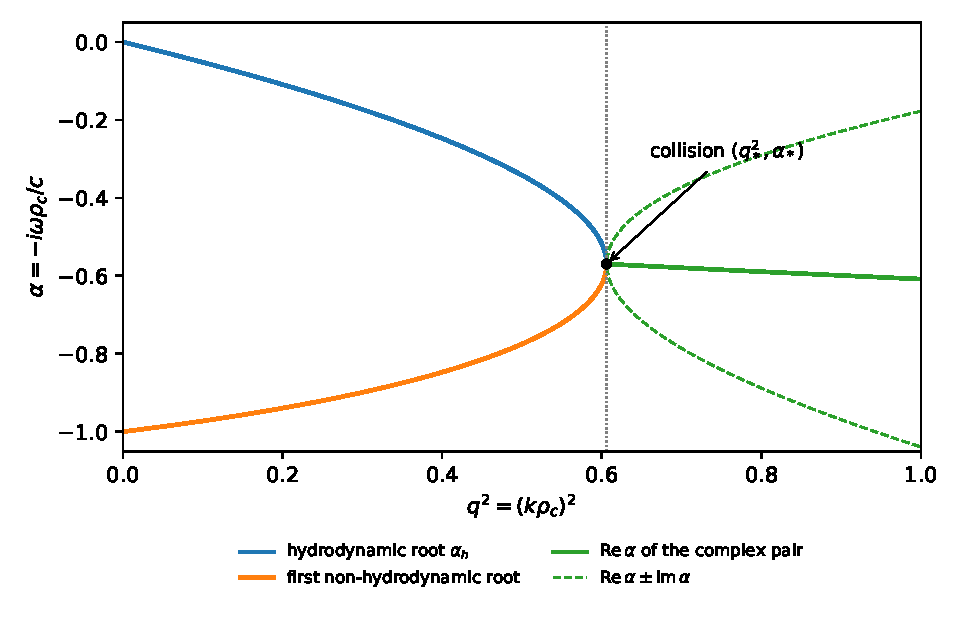
\includegraphics[width=0.86\linewidth]{fig_ns_collision.pdf}
\caption{The real zeros of $\alpha\mapsto I'_\alpha(q)$ near the collision, computed with mpmath (the figure's script is in the paper's source folder). For $q^2<q_*^2=0.60602\ldots$ the hydrodynamic root $\alpha_h$ and the first non-hydrodynamic root are real and distinct; they meet at $(q_*^2,\alpha_*)$ in a square-root fold (Theorem~\ref{thm:collision}), and beyond it they form a complex-conjugate pair, shown by its real part and by $\re\alpha\pm\im\alpha$. The figure is an illustration; the statements are certified in Theorems~\ref{thm:collision} and~\ref{thm:radius}.}
\label{fig:collision}
\end{figure}

\subsection{The collision}

\begin{theorem}[the collision]\label{thm:collision}
There is $(\alpha_*,q_*)$ with
\begin{gather*}
|q_*-0.778472800990330076180356446189|<10^{-20},\\ |\alpha_*+0.569714080972361784438457668663|<1.5\cdot10^{-10},
\end{gather*}
at which $F=F_\alpha=0$. At that point $F_q\in1.75035806\pm7.6\cdot10^{-9}$ and $F_{\alpha\alpha}\in5.00\pm0.0203$, both positive. So the two roots meet in a square-root fold: they are real for $q<q_*$ near $q_*$ and complex conjugate for $q>q_*$ near $q_*$.
\end{theorem}
\status{Proved here with computer assistance, in Arb ball arithmetic through python-flint. The program is \note{first\_pass/\allowbreak certify\_collision.py}; it was read line by line and re-run.}
\begin{proof}
Let $I=a_0\pm1.5\cdot10^{-10}$ and $J=q_0\pm10^{-20}$ with the centres displayed above. Ball arithmetic shows:
\begin{enumerate}[label=(\roman*)]
\item $F>0$ on $\partial I\times J$;
\item $F(a_0,q_0-10^{-20})<0$;
\item $F>0$ on $I\times\{q_0+10^{-20}\}$.
\end{enumerate}
The function $g(q)=\min_{\alpha\in I}F(\alpha,q)$ is continuous, with $g(q_0-10^{-20})<0<g(q_0+10^{-20})$. At a zero $q_*$ of $g$ the minimiser $\alpha_*$ is interior to $I$ by (i), so $F=F_\alpha=0$ there. By the Bessel equation, $F_q=I''_\alpha(q)=(1+\alpha^2/q^2)I_\alpha-I'_\alpha/q$, which is enclosed directly; $F_{\alpha\alpha}$ is enclosed by a divided difference with a Cauchy remainder, the maximum modulus being taken on a circle of radius $0.05$. Since $F_q\ne0$ and $F_{\alpha\alpha}\ne0$, the two roots split as a square root in $q-q_*$.
\end{proof}

\subsection{The radius, exactly}

\begin{theorem}[the radius of the hydrodynamic series]\label{thm:radius}
Let $x_*=q_*^2/4$.
\begin{enumerate}[label=(\alph*)]
\item The hydrodynamic root $\alpha_h$ continues analytically to the open disk $|x|<x_*$. It is real and negative for $0<x<x_*$, so the shear mode is purely damped there.
\item As $x\uparrow x_*$ along the reals, $\alpha_h(x)\to\alpha_*$, and $\alpha_h$ has a square-root branch point at $x_*$.
\item The Taylor series of $\alpha_h$ in $x$ has radius of convergence exactly $x_*$. Equivalently, the series in $q^2$ has radius exactly $q_*^2=0.6060199018817300556\pm5.3\cdot10^{-20}$; in physical units $\omega(k)$ has radius exactly $k_*=q_*c/(2\nu)=0.389236400495165038\ldots\,c/\nu$ in $k$, and its first singularity is $\omega_*=-0.2848570405\ldots\,i\,c^2/\nu$.
\item For real $x$ slightly above $x_*$ the two roots near $\alpha_*$ are complex conjugates: the modes propagate.
\end{enumerate}
\end{theorem}
\status{Proved here with computer assistance (\note{certify\_hydro\_radius.py}, certified in $137$\,s). Independently re-verified by the referee: all Krawczyk conditions with a second interval library (\texttt{mpmath.iv}, $36$ terms, an independently derived tail bound), coverage and all consistency pairs in exact integer arithmetic, and the fold patch at twice the resolution.}
\begin{proof}
Every step is a finite ball-arithmetic computation.

\emph{Rigorous evaluation.} $G$ and $G_\alpha$ are summed to $M=30$ terms in Arb. For $|\alpha|\le a=0.95$ and $|x|\le X=0.2$ the terms satisfy $|t_m|\le b_m:=(a+2m)X^m/\bigl(m!\prod_{k\le m}(k-a)\bigr)$ and $|\partial_\alpha t_m|\le d_m:=X^m/\bigl(m!\prod_{k\le m}(k-a)\bigr)\cdot\bigl(1+(a+2m)\sum_{k\le m}1/(k-a)\bigr)$. For $m\ge30$, $b_{m+1}/b_m\le2X/((m+1)(m+1-a))\le\frac12$ and $d_{m+1}/d_m\le5X/((m+1)(m+1-a))\le\frac12$, so the tails are at most $2b_M$ and $2d_M$; they are added to the ball radii.

\emph{The Krawczyk tiling.} The closed disk $|x|\le R_{\mathrm{hi}}$, with $R_{\mathrm{hi}}\ge x_*$ the upper end of the certified box, minus the open square of half-width $3\cdot2^{-10}$ about a centre $X_c=x_*+O(3\cdot10^{-8})$, is covered by $42{,}650$ square cells, subdivided adaptively $3\times3$. For each cell $X_i$ and a square $\alpha$-box $A_i$ with centre $c$ and a real scalar $Y$, the Krawczyk operator
\[
K_i=c-YG(c,X_i)+\bigl(1-YG_\alpha(A_i,X_i)\bigr)(A_i-c)
\]
lies in the interior of $A_i$.
\begin{itemize}
\item \emph{Existence.} $A_i$ is convex and $G$ is analytic in $\alpha$. By the mean-value integral $G(\alpha,x)-G(c,x)=\int_0^1G_\alpha(c+t(\alpha-c),x)\,dt\cdot(\alpha-c)$, whose integral lies in the convex enclosure of $G_\alpha(A_i,X_i)$, the map $N_x(\alpha)=\alpha-YG(\alpha,x)$ sends $A_i$ into $K_i\subset A_i$ for every $x\in X_i$. Brouwer's theorem gives a fixed point, which is a zero because $Y\ne0$.
\item \emph{Uniqueness and simplicity.} Two zeros in $A_i$, or a zero of $G_\alpha$ in $A_i$, would put $0$ in the convex hull of $G_\alpha(A_i,x)$. Then $1\in1-YG_\alpha(A_i,X_i)$, and $K_i$ would contain the translate $c-YG(c,x)+(A_i-c)$ of $A_i$, which cannot lie in the interior of $A_i$.
\item So for every $x\in X_i$ there is exactly one zero in $A_i$; it is simple, lies in $K_i$ and is analytic in $x$. The cells are enlarged by the factor $1+10^{-9}$, so that the rounding of cell centres leaves no gaps, and every wanted cell is certified or subdivided, with no failures.
\end{itemize}

\emph{Consistency.} On all $168{,}301$ touching pairs, $K_i\subseteq A_j$ or $K_j\subseteq A_i$, so the unique zeros agree on the overlaps. The cells containing $x=0$ contain $\alpha=0$. So the zeros form one analytic function on the tiled region, the continuation of $\alpha_h$.

\emph{Realness.} The $102$ cells that meet the real axis have real centres and real-symmetric $\alpha$-boxes, and uniqueness forces the zero to be real for real $x$.

\emph{The fold patch.} Let $A_F$ be the square of half-width $\frac14$ about a dyadic $\alpha_0\approx\alpha_*$, and $X_F$ the square of half-width $2^{-8}$ about $X_c$; all corners and boundary points are exact binary numbers.
\begin{enumerate}[label=(F\alph*)]
\item $G\ne0$ on $\partial A_F\times X_F$, with $\min|G|\ge0.0774$.
\item The winding number of $G(\cdot,X_c)$ along $\partial A_F$ is $2$ (enclosure $2.00000\pm3\cdot10^{-10}$). So for every $x\in X_F$, $G(\cdot,x)$ has exactly two zeros $\beta_1,\beta_2$ in $A_F$, counted with multiplicity, and their discriminant $\Delta=(\beta_1-\beta_2)^2=2p_2-p_1^2$, with $p_k=(2\pi i)^{-1}\oint_{\partial A_F}\alpha^kG_\alpha/G\,d\alpha$, is analytic on $X_F$.
\item On the $256$ boundary segments of $X_F$ the two zeros lie in disjoint Krawczyk boxes inside $A_F$, and the winding number of $\Delta$ along $\partial X_F$ is $1$ (enclosure $1.00000\pm3\cdot10^{-11}$). So $\Delta$ has exactly one zero in $X_F$, and it is simple. That zero is $x_*$, because Theorem~\ref{thm:collision} places the double zero $(\alpha_*,x_*)$ in $A_F\times X_F$.
\item All $4{,}039$ tiled cells that meet $X_F$ have $K_i\subseteq A_F$, so there $\alpha_h$ is one of $\beta_1,\beta_2$.
\end{enumerate}

\emph{Conclusion (a).} On $X_F\cap\{|x|<x_*\}$, a convex set with $x_*$ on its boundary, $\Delta\ne0$, so $\beta_1$ and $\beta_2$ are distinct and each is analytic there. The tiled function equals one of them on the connected set formed by the tiled region, $X_F$ and the disk $\{|x|<x_*\}$: this set contains the part of the square annulus between the half-widths $3\cdot2^{-10}$ and $2^{-8}$ that lies inside the disk, and the circle $|x|=x_*$ passes through the central hole. So $\alpha_h$ is analytic on $|x|<x_*$. On the real segment $[X_c-2^{-8},x_*)$, $\alpha_h$ is real at a tiled point, so its partner is real too, $\Delta$ is real and nonzero, and it is positive at the tiled end; hence $\Delta>0$ and both zeros are real up to $x_*$. Finally $G(0,x)=\sum_m2m\,x^m/(m!)^2>0$ for $x>0$, so $\alpha=0$ is never a zero for $x>0$; since $\alpha_h$ is real and continuous with $\alpha_h'(0)=-2$, it stays negative on $(0,x_*)$, and the frequency $w=i\alpha_h$ is negative imaginary.

\emph{Conclusions (b) and (d).} Near $x_*$ the two zeros are $(p_1\pm\sqrt\Delta)/2$ with a simple zero of $\Delta$ at $x_*$, and $\alpha_h\to p_1(x_*)/2=\alpha_*$ as $x\uparrow x_*$. If $\alpha_h$ were analytic at $x_*$, then $\sqrt\Delta=\pm(2\alpha_h-p_1)$ would be analytic there, and $\Delta$ would have a zero of even order. For real $x>x_*$ near $x_*$, $\Delta<0$, since the zero is simple and $\Delta>0$ to its left; so the two zeros are a conjugate pair.

\emph{Conclusion (c).} A power series at $0$ with radius $R>x_*$ would agree with $\alpha_h$ on $|x|<x_*$ and be analytic at $x_*$, contradicting (b); the radius is at least $x_*$ by (a). The physical constants follow from $k=q/\rho_c=qc/(2\nu)$ and $\omega=i\alpha c/\rho_c$.
\end{proof}

The fold patch gives two further facts. The collision is the only branch point of the two roots in $A_F\times X_F$, and it is nondegenerate independently of the enclosures of $F_q$ and $F_{\alpha\alpha}$ in Theorem~\ref{thm:collision}. And the partner root is certified real, simple and distinct from $\alpha_h$ on $[X_c-2^{-8},x_*)$. As a negative control, the same tiling asked to cover the disk $|x|\le0.158>x_*$ fails on the real axis beyond $x_*$, from $x=0.15451$, as it must: there the two zeros are a conjugate pair, which no real-symmetric box can isolate.

\subsection{The coefficients and the sum on the circle}

\begin{corollary}[coefficient asymptotics and boundary sum]\label{cor:darboux}
Write $\alpha_h(x)=\sum_{k\ge1}a_kx^k$. Then
\[
a_k=-C\,x_*^{-k}\,k^{-3/2}\bigl(1+O(1/k)\bigr),\qquad C=\frac{\kappa\sqrt{x_*}}{2\sqrt\pi},\qquad \kappa^2=\frac{4F_q}{q_*F_{\alpha\alpha}}.
\]
The enclosures of Theorem~\ref{thm:collision} give $\kappa^2\in[1.7915,1.8061]$ and $C\in[0.14696,0.14757]$; numerically $\kappa=1.3403764770$ and $C=0.1471754300$. In particular $a_k<0$ for all sufficiently large $k$. The series converges absolutely on $|x|=x_*$, and $\sum_ka_kx_*^k=\alpha_*$: the dispersion series summed at $k=k_*$ equals the collision frequency $\omega_*$.
\end{corollary}
\status{Proved here with computer assistance; the numerical value of $C$ uses $F_{\alpha\alpha}$ to $30$ digits (RESEARCH.md (32)). The sign $\kappa>0$ is certified in \note{ns51\_sign\_check.py}.}
\begin{proof}
\emph{A $\Delta$-domain.} Every closed tiled cell carries a simple zero, so by the implicit function theorem and compactness $\alpha_h$ extends to an open neighbourhood of the tiled region. The fold square $X_F$ is a full neighbourhood of $x_*$, on which the two zeros are $(p_1\pm\sqrt\Delta)/2$ with $\Delta\ne0$ off $x_*$. Hence $\alpha_h$ is analytic and single-valued on a slit disk $\{|x|<x_*+\varepsilon\}\setminus[x_*,x_*+\varepsilon)$ for some $\varepsilon>0$, which contains a $\Delta$-domain at $x_*$ in the sense of singularity analysis.

\emph{The local expansion.} Near $x_*$, $\alpha_h=(p_1+\sqrt\Delta)/2$ with $p_1$ and $\Delta$ analytic and $\Delta(x_*)=0$ simple, and the quadratic model of $F$ at the fold gives $\Delta=4\kappa^2(x_*-x)(1+O(x_*-x))$. Hence
\[
\alpha_h=\alpha_*+\kappa\sqrt{x_*}\,(1-x/x_*)^{1/2}+c_1(x_*-x)+c_2(x_*-x)^{3/2}+\cdots.
\]
The sign $\kappa>0$ holds because the hydrodynamic zero is the upper of the two real zeros on $[X_c-2^{-8},x_*)$. This is certified by a chain of $400$ real Krawczyk cells that continues $\alpha_h$ from $\alpha=0$ at $x=0$ to $x_0=X_c-2^{-8}$, where it lies in $[-0.526,-0.474]$; the two fold zeros at $x_0$ are enclosed in $-0.484383876487\pm1.2\cdot10^{-13}$ and $-0.651760880396\pm4\cdot10^{-13}$, and the chain's enclosure meets only the upper one.

\emph{Transfer.} By the transfer theorem of singularity analysis \cite{FlajoletOdlyzko}, $[z^k](1-z)^{1/2}=-k^{-3/2}/(2\sqrt\pi)\,(1+O(1/k))$; the analytic term $c_1(x_*-x)$ contributes nothing for $k\ge2$, and $(x_*-x)^{3/2}$ contributes $O(k^{-5/2})$. This gives the asymptotics, and $a_kx_*^k=O(k^{-3/2})$ gives absolute convergence on the circle. Abel's theorem and $\alpha_h(x)\to\alpha_*$ as $x\uparrow x_*$ give the boundary sum.
\end{proof}

The first $240$ Taylor coefficients were computed exactly as rationals, with $G(\alpha_h(x),x)=O(x^{241})$ checked exactly (\note{hydro\_series.py}):
\[
a_1=-2,\ a_2=-3,\ a_3=-\tfrac{29}3,\ a_4=-\tfrac{2843}{72},\ a_5=-\tfrac{392029}{2160},\ a_6=-\tfrac{14509367}{16200},\ a_7=-\tfrac{63074754607}{13608000}.
\]
They reproduce the continuation's series in $q^2=4x$, including its fifth coefficient. All $240$ are negative, and the referee extended this to $320$. The Darboux-corrected ratios $(a_k/a_{k+1})/(1+3/(2k))$ approach $x_*=0.1515049754\ldots$ with error $O(1/k^2)$: $0.15158$ at $k=40$, $0.151517$ at $k=100$ and $0.1515080$ at $k=200$. From the referee's $320$ coefficients, $a_kx_*^kk^{3/2}\to-0.147175429969$ by Richardson extrapolation, which is $-C$ to $12$ digits; the partial sum $S_{320}$ plus the Darboux tail equals $\alpha_*$ to $1.6\cdot10^{-11}$; and the fold-patch discriminant has $\Delta'(x_*)=-7.186436=-4\kappa^2$.
\status{Checked numerically.}

\subsection{The other modes, and the physical reading}

The root that collides with $\alpha_h$ is the first non-hydrodynamic mode. Followed backwards in $\alpha$ from $\alpha_*$ (near the fold, $q$ is a smooth function of $\alpha$, since $F_q\ne0$), it reaches $q\to0$ as $\alpha\to-1$ with $x\approx1+\alpha$ (\note{track\_partner.py}; numerical). As $q\to0$ the zeros of $\alpha\mapsto I'_\alpha(q)$ tend to the zeros of $1/\Gamma(\alpha)$, namely $\alpha=0,-1,-2,\dots$: indeed
\[
2(q/2)^{1-\alpha}I'_\alpha(q)=\sum_m\frac{(2m+\alpha)(q/2)^{2m}}{m!\,\Gamma(m+\alpha+1)}\longrightarrow\frac{\alpha}{\Gamma(\alpha+1)}=\frac1{\Gamma(\alpha)}
\]
locally uniformly in $\alpha$, and Hurwitz's theorem applies. (At $q=0$ itself the boundary problem degenerates, so the statement is a limit.) The referee found numerically that $(\alpha+n)/q^{2n}\to(-1)^{n+1}n/((n!)^24^n)$ for $n=1,2,3$. The cutoff observer has proper acceleration $c^2/\rho_c$ and redshift factor $1$ at $\rho=\rho_c$, so its Unruh temperature is $T=\hbar c/(2\pi k_B\rho_c)$, and the non-hydrodynamic frequencies tend to $\omega_n=-inc/\rho_c=-2\pi inT$ (units $\hbar=k_B=1$): the Matsubara frequencies.

\begin{itemize}
\item \emph{Normalisation.} With $2\pi T=c/\rho_c$, $(w,q)=(\omega,ck)/(2\pi T)$ are exactly the dimensionless variables $(\mathfrak w,\mathfrak q)$ of Grozdanov, Kovtun, Starinets and Tadić \cite{GKST}. The collision is a critical point of the spectral curve $F(\alpha,q)=0$ at real $\mathfrak q_*^2=0.6060199$ and imaginary $\mathfrak w_*=-0.5697141\,i$, and Theorem~\ref{thm:radius} is the flat-cutoff instance of their statement that the radius of the hydrodynamic series is set by the nearest critical point of the spectral curve on the hydrodynamic sheet. Here that critical point lies at real momentum.
\item \emph{Shear viscosity.} $\rho_c=2\nu/c$ gives $\nu=c^2/(4\pi T)$. With $\eta=\nu(\varepsilon+p)/c^2$ and $\varepsilon+p=Ts$ at zero chemical potential, $\eta/s=\nu T/c^2=1/(4\pi)$ in units $\hbar=k_B=1$.
\item \emph{Pole collisions.} Areán, Davison, Goutéraux and Suzuki characterise the breakdown of diffusion near AdS$_2$ critical points by a collision of the diffusive pole with a non-hydrodynamic pole \cite{ADGS}; the same kind of event bounds the series here. At the collision, $|\omega_*|/(\nu k_*^2)=|\alpha_*|/(q_*^2/2)=1.8802$, so at the radius the leading diffusive law is off by a factor $1.88$.
\item \emph{The $k^4$ coefficient.} Compère, McFadden, Skenderis and Taylor write the corrected Rindler Navier--Stokes equation \cite[(6.3)]{CMST}; its linear part is $\partial_\tau v-r_c\partial^2v=-\frac32r_c^2\partial^4v$ in their time $\tau$, with induced metric $-r_c\,d\tau^2+dx^2$. In proper time $t=\sqrt{r_c}\,\tau$ and velocity $v/\sqrt{r_c}$ this becomes $\partial_tv-\sqrt{r_c}\,\partial^2v=-\frac32r_c^{3/2}\partial^4v$, so $\nu=\sqrt{r_c}$ and $\omega=-i\nu k^2-\frac32i\nu^3k^4$ ($c=1$), which is the second coefficient above. (Only the linear terms of (6.3) were read, through a text extraction.) The $k^6$ coefficient and all higher ones come from the exact condition \eqref{eq:disp}.
\item \emph{A two-pole model.} The telegraph model $w^2+iw-q^2/2=0$, that is $\alpha^2+\alpha+2x=0$, calibrated to the diffusion constant and to the first non-hydrodynamic mode, collides at $x=\frac18$ ($q^2=\frac12$) and $\alpha=-\frac12$, with hydrodynamic branch $-2x-4x^2-16x^3-\cdots$. The exact problem moves the collision to $(q_*^2,\alpha_*)=(0.6060,-0.5697)$, with branch $-2x-3x^2-\frac{29}3x^3-\cdots$.
\end{itemize}
\status{The Unruh temperature, the normalisation and $\eta/s$ are derived here; the comparisons with \cite{GKST,ADGS} are readings of those papers' abstracts and statements, not re-derivations.}

A statement of the Rindler radius was not found in \cite{BKLS,CMST,MarolfRangamani,GKST,Withers,HSSSW}; that check was made through their abstracts and text excerpts, and the search was not exhaustive.

\section{Curvature rates for the map to Yang--Mills}\label{sec:rates}

The Yang--Mills repository maps a velocity field $u$ to the abelian connection $A_i=\lambda u_iT$ (the Yang--Mills paper \cite{YMPaper}, Section~6), whose curvature masses are
\[
\mathcal K_B=\lambda^2\|\operatorname{curl}u\|^2,\qquad \mathcal K_E=\lambda^2c^{-2}\|\partial_tu\|^2,
\]
and it derives lower rates for them from the manuscript's profile estimates (\texttt{ns\_inner\_\allowbreak profile\_\allowbreak curvature\_\allowbreak current\_\allowbreak bridge.md}, §§4--5, in \texttt{yang-mills/\allowbreak sources/\allowbreak ym\_gap\_primary\_20260908/}). The rates are derived from named statements of the manuscript, and every step of the derivation was re-derived here, so their status is \emph{conditional} on those statements.

\subsection{The four statements used}

All four are statements of the manuscript and are imported.
\begin{itemize}
\item[(H1)] Theorem~4.6(i) (src p.~33): $E=\sqrt{2X}F>0$ for $X>0$ and every $\eta\in[-1,1]$, with $F=\varphi/\mathsf C$ smooth on $[0,R]\times[-1,1]$. In particular $E_0>0$ on the inner region, and $E_0(X,\eta)=O(\sqrt X)$ at the axis.
\item[(H2)] Proposition~5.5, (5.42) (src p.~60): for every composition $\mathcal D^I$ of $q\partial_q$, $\partial_X$ and $\partial_\eta$, $\mathcal D^I(q^Au_{\theta,B}-E_0)=O(q^{2h})$ uniformly on $[X_{\mathrm{lo}},X_{\mathrm{hi}}]\times[-1,1]$. The source fixes radial endpoints $0<X_{\mathrm{lo}}<X_a<X_b<X_{\mathrm{hi}}$ and lets the constants depend on them; this is read as holding for each such choice, as the bridge file reads it. It holds for the summed background, with the Stokes streamfunctions summed before differentiation, so the summation cutoffs are already included.
\item[(H3)] All annular corrections vanish on the fixed inner similarity region $X\in(0,X_a)$, for every $\eta$. Step~5 of Proposition~9.9 (src p.~116) says this at the chosen point $X_{\mathrm{in}}$; the region-wide statement is the sentence after (10.21) on src p.~124, and it is also carried by the support statement of Theorem~4.6(ii), by which the stress vanishes for $X\le X_a$.
\item[(H4)] Proposition~10.1: the cutoffs equal one on a neighbourhood of the singular point.
\end{itemize}

\subsection{The rates}

\begin{theorem}[curvature rates]\label{thm:rates}
Under (H1)--(H4), for every $\nu>0$ there are $C_\Omega,C_{\dot u}>0$ such that for all small $\tau=1-t$
\[
\|\operatorname{curl}u_\nu(1-\tau)\|_2^2\ge\nu^{3/2}C_\Omega\,\tau^{-1/2-3h},\qquad \|\partial_tu_\nu(1-\tau)\|_2^2\ge\nu^{5/2}C_{\dot u}\,\tau^{-3/2-3h}.
\]
Hence, for the abelian image $A_i=\lambda u_{\nu,i}T$, $\mathcal K_B(1-\tau)\to\infty$ while $\int_0^1\mathcal K_B\le\lambda^2\mathcal F_\nu(1)^2/(2\nu)<\infty$, and $\mathcal K_E(1-\tau)\to\infty$ with $\int_0^1\mathcal K_E=\infty$.
\end{theorem}
\status{\textsf{Conditional} on (H1)--(H4); every step re-derived, and every exponent computation checked symbolically, with three negative controls (\note{ns51\_rate\_lemmas.py}, $27$ checks).}
\begin{proof}
Choose $X_*\in(X_{\mathrm{lo}},X_a)$ with $e_0=E_0(X_*,0)>0$, and $\eta_*>0$ with $E_0(X_*,\eta)\ge e_0/2$ for $|\eta|\le\eta_*$. By (H2)--(H4), $u_\theta\ge(e_0/4)q^{-A}$ on the circles $r=\sqrt{2X_*q}$, $|\eta|\le\eta_*$, for small $\tau$.

\emph{Enstrophy.} On the disk $D_z$ bounded by such a circle, Stokes' theorem gives $\int_{D_z}\omega_3=2\pi r u_\theta$, and Cauchy--Schwarz gives $\int_{D_z}\omega_3^2\ge(2\pi ru_\theta)^2/(\pi r^2)=4\pi u_\theta^2$. At fixed $\tau$, $dz/d\eta=\tau^D(1-2h\eta^2)(1-\eta^2)^{-D-1}$, and integrating over $|\eta|\le\eta_*$ gives the enstrophy bound with the exponent $D-2A=-\frac12-3h$.

\emph{The time derivative.} At a fixed point, $q_t=-1/L$, $\eta_t=D\eta/(qL)$ and $X_t=X/(qL)$ with $L=1-2h\eta^2$. So $\partial_tu_\theta=q^{-A-1}\bigl(\mathcal H+O(q^{2h})\bigr)$ with $\mathcal H=(AE+XE_X+D\eta E_\eta)/L$. By (H1), $E=\sqrt{2X}F$ gives $\mathcal H(X,0)=(1+h)E(X,0)+O(X^{3/2})>0$ for small $X>0$. Integrating over a rectangle on which $|\mathcal H|\ge h_*>0$, with the volume element $dx=q\tau^DL(1-\eta^2)^{-D-1}\,dX\,d\theta\,d\eta$, gives the exponent $D-2A-1=-\frac32-3h$.

\emph{Finiteness of $\int\mathcal K_B$.} The energy inequality $\|u\|^2+2\nu\int\|\nabla u\|^2\le\mathcal F_\nu(t)^2$ and $\|\operatorname{curl}u\|=\|\nabla u\|$ for divergence-free, compactly supported fields give $\int_0^1\mathcal K_B\le\lambda^2\mathcal F_\nu(1)^2/(2\nu)$.

\emph{Viscosity scaling.} The viscosity map (10.22) gives the factors $\nu^{3/2}$ and $\nu^{5/2}$.
\end{proof}

\subsection{Type II blowup and the growth of the critical norm}

\begin{proposition}[Type II and critical-norm growth]\label{prop:typeII}
Under (H1)--(H4), for small $\tau$:
\begin{enumerate}[label=(\alph*)]
\item $\|u(1-\tau)\|_p^p\ge c_p\,\tau^{3/2-h-p(1/2+h)}$ for every $1\le p<\infty$. The exponent is negative exactly for $p>p_h=(3-2h)/(1+2h)$, and $p_h<3$. In particular $\|u(1-\tau)\|_{L^3}\ge c\,\tau^{-4h/3}\to\infty$, and the lower bound diverges also for $p_h<p<3$, although these norms are subcritical; for $p=2$ the norm stays bounded by the energy inequality, and the core contribution decays like $\tau^{1/2-3h}$ (src p.~4).
\item $\|\omega(1-\tau)\|_\infty\ge c\,\tau^{-1-h}$, from a disk mean away from the axis.
\item $\tau^{1/2}\|u(1-\tau)\|_\infty\ge c\,\tau^{-h}\to\infty$. So the blowup is not of Type~I, $|u|\le C(T-t)^{-1/2}$: it is of Type~II.
\end{enumerate}
\end{proposition}
\status{\textsf{Conditional} on (H1)--(H4); the exponent algebra checked in \note{ns51\_rate\_lemmas.py}.}
\begin{proof}
(a) Integrate $|u_\theta|^p\ge(e_0/4)^pq^{-pA}$ over a rectangle as in the proof of Theorem~\ref{thm:rates}; the $\tau$-exponent is $1+D-pA$. For $p=3$ the $\eta$-factor is $L(1-\eta^2)^{-1+4h}$, which is integrable on compact $\eta$-sets.
(b) The mean of $\omega_3$ on the disk $D_z$ is $2u_\theta/r\ge\sqrt2(e_0/4)X_*^{-1/2}q^{-1-h}$, and the maximum dominates the mean. The disk has radius $\sqrt{2X_*q}$, away from the axis, where (5.42) is not available, so no axis information is needed.
(c) Use the growth path (10.21) with $q=\tau$.
\end{proof}

\emph{Comparison with the classical necessary conditions for a singularity.} Each of them is satisfied. The margins stated are lower bounds only, since no matching upper bounds are established here.
\begin{itemize}
\item \emph{Leray's rates} \cite{Leray}. A singular time forces $\|\nabla u(t)\|_2^2\gtrsim(T-t)^{-1/2}$, and $\|u(t)\|_p\gtrsim(T-t)^{-(p-3)/(2p)}$ for $p>3$; Robinson, Sadowski and Silva discuss these lower bounds \cite{RSS}. The enstrophy exponent here is $\frac12+3h$, a margin of $\tau^{-3h}$, and $\int\tau^{-1/2-3h}<\infty$ exactly when $h<\frac16$, as the finite dissipation requires. For $p>3$ the margin is $\tau^{-h(1+1/p)}$, and as $p\to\infty$ this becomes (c).
\item \emph{The $L^3$ criterion.} Escauriaza, Seregin and Šverák prove regularity under a bound in $L^\infty_tL^3_x$ for the unforced Cauchy problem \cite{ESS}, and Seregin shows that $\|u(t)\|_{L^3}\to\infty$ at a potential blowup time \cite{Seregin}. Here $\|u\|_3\gtrsim\tau^{-4h/3}$ diverges. These criteria require divergence, not a rate, and whether they extend verbatim to smooth compactly supported forcing was not checked, so this is a statement of consistency, not of implication.
\item \emph{Axisymmetric Type~I exclusion.} Chen, Strain, Tsai and Yau \cite{CSTY} and Koch, Nadirashvili, Seregin and Šverák \cite{KNSS} exclude Type~I blowup for axisymmetric unforced solutions. The construction here is axisymmetric only on its inner region (H3), and the equation is forced, so those theorems do not apply as stated. Proposition~\ref{prop:typeII}(c) shows that it exceeds the Type~I rate by at least the factor $\tau^{-h}$, the angular Reynolds number of src p.~4.
\item \emph{$L^2_tL^\infty_x$ and $\int\|\omega\|_\infty$.} $\int\|u\|_\infty^2\gtrsim\int\tau^{-1-2h}=\infty$ and $\int\|\omega\|_\infty\gtrsim\int\tau^{-1-h}=\infty$, with margins $\tau^{-2h}$ and $\tau^{-h}$ against the scaling rates. These divergences hold for every singular solution, by Leray's bound $\|u(t)\|_\infty\gtrsim(T-t)^{-1/2}$ and by criteria of Beale--Kato--Majda type, so only the exponent arithmetic is claimed.
\end{itemize}

\subsection{A formula of the growth path}

The official PDF of the manuscript prints (10.20) as $x_\tau=(\sqrt{2X_{\mathrm{in}}\tau},0,0)$, with the radical over $2X_{\mathrm{in}}\tau$ (checked on p.~124 of the PDF whose hash the transcription freezes). With this path, $q=\tau$ and $X=X_{\mathrm{in}}$, and (10.21) follows from (3.6). The workbench's transcription renders the radical over the factor $2$ only; on that path $X=X_{\mathrm{in}}^2\tau\to0$ and $u_\theta$ would grow only like $\tau^{-h}$. So the source is correct, and the transcription's errata ledger, which was empty, gets this correction as its first entry.
\status{Verified against the official PDF.}

\section{Proved limits}\label{sec:negative}

Three statements of the preceding sections are limits, and each is proved.
\begin{itemize}
\item \emph{The dispersion series does not converge beyond $k_*$} (Theorem~\ref{thm:radius}(c)). A series with a larger radius would make $\alpha_h$ analytic at $x_*$, where it has a square-root branch point. The negative control confirms this: the same tiling, asked to cover the disk of radius $0.158>x_*$, fails on the real axis beyond $x_*$, where the two zeros are a conjugate pair.
\item \emph{Beyond the collision the shear modes propagate} (Theorem~\ref{thm:radius}(d)). For real $x$ slightly above $x_*$ the two roots near $\alpha_*$ are complex conjugates, so the purely damped regime ends exactly at $k_*$.
\item \emph{The two-pole model misplaces the collision.} The telegraph model $\alpha^2+\alpha+2x=0$, calibrated to the diffusion constant and to the first non-hydrodynamic mode, collides at $(q^2,\alpha)=(\frac12,-\frac12)$, while the exact collision is at $(0.6060,-0.5697)$. So the radius is a property of the exact dispersion relation and is not captured by the two-pole truncation.
\end{itemize}
The rates of Section~\ref{sec:rates} carry a limit of scope that the workbench states itself: the zero-quotient sequence of the map to Yang--Mills exists only along couplings $g_j\to0$, and it rests on (H1)--(H4).

\section{The typed maps to the other programmes}\label{sec:bridges}

The workbench connects the Navier--Stokes construction to the author's other programmes through explicit maps. The table states what each map carries and what is established about it here; \emph{verified} marks an identity or a statement re-derived here.

\begin{center}\small
\begin{longtable}{@{}>{\raggedright\arraybackslash}p{0.2\linewidth}>{\raggedright\arraybackslash}p{0.36\linewidth}>{\raggedright\arraybackslash}p{0.36\linewidth}@{}}
\toprule
Map & What it carries & Established here\\
\midrule
\endhead
NS $\to$ YM, abelian & $A_i=\lambda u_iT$; the curvature masses $\mathcal K_B=\lambda^2\|\operatorname{curl}u\|^2$ and $\mathcal K_E=\lambda^2c^{-2}\|\partial_tu\|^2$ & the map and its identities, verified; the divergence of the curvature masses conditional on (H1)--(H4) (Theorem~\ref{thm:rates}); the zero-quotient diagonal needs couplings $g_j\to0$\\
NS $\to$ YM, non-abelian & $\mathbf A_i=\lambda e_i\times u$; its fields, invariants and currents & all identities verified for every divergence-free $u$; the off-axis vorticity bound of Proposition~\ref{prop:typeII}(b) under (H1)--(H4). The exact axis identity of the source's (243) comes from the workbench's own axis continuation, not from (H1)--(H4), since (5.42) does not reach the axis. The current is nonzero, so the image is a sourced field\\
NS $\to$ Erdős--Straus & the auxiliary torus operator $J=\begin{psmallmatrix}3&1\\1&5\end{psmallmatrix}$, with $\det J=14$ and eigenvalues $4\pm\sqrt2$ & the operator identities used in $21$ statements of the Erdős--Straus supplement, verified in the Erdős--Straus paper \cite{ESPaper}\\
NS $\to$ zeta & angular-momentum balance, a Mellin shift and the Müntz multiplier $W_h(s)=\zeta(s)(1-2^{s-1})(1-2^{h-s})$ & the transforms, verified; the growth, conditional on Theorem~\ref{thm:rates}; the Mellin abscissa of $\mathcal K_B(1-\tau)$ lies in $[\frac12+3h,1]$, conditionally\\
$S^6\to$ NS & a Beltrami-mode forced solution on $\mathbb T^3$ from the $S^6$ oscillator & a global smooth solution, verified exactly\\
Jacobian map $\to$ NS kinematics & $U=DF^{-1}(V\circ F)$, a divergence-free polynomial field whose flow escapes at $\tau=1/8$ & verified exactly (the Jacobian paper \cite{JacobianPaper}, §4)\\
NS $\to$ Einstein & the snapshot encoding, the Kasner map, the Rindler response and the slab comparator & all identities verified; the collision and the exact radius of Section~\ref{sec:rindler}\\
\bottomrule
\end{longtable}
\end{center}

My assessment of these maps, taken together: the map to Einstein gravity has produced the strongest result so far, the exact radius of Section~\ref{sec:rindler}. I think it is of independent interest in fluid/gravity duality, because it places the breakdown of the hydrodynamic expansion of the Rindler fluid at a certified pole collision at real momentum, a question the continuation had left open. The maps to Yang--Mills are exact as identities, and their analytic content is conditional on (H1)--(H4); certifying those four statements (Question~\ref{q:profiles}) would make the curvature rates unconditional. For the maps to the zeta programme and to the Erdős--Straus workbench, what is established is the exact identities; what they carry about the zeta function or the equation beyond those identities is not verified here.

The connections to established work are these: the convergence of the hydrodynamic gradient expansion \cite{GKST,Withers,HSSSW}; the breakdown of diffusion by pole collision \cite{ADGS}; fluid/gravity duality and the Rindler fluid \cite{BHMR,BKLS,CMST,MarolfRangamani}; forced singularities, whose strategy of the force as a residual with controlled regularity the manuscript shares \cite{CordobaMartinezZoroa}; the classical blowup criteria of Section~\ref{sec:rates}; and singularity analysis of power series \cite{FlajoletOdlyzko}. The manuscript's Lemma~10.3 is, in its structure, Borel's lemma with shrinking cutoffs (a reading of the first pass), and its exterior heat profile $\mathcal H(Z)=Z^{-1-h}U(1+h,2,1/Z)$ is a Tricomi function (verified in \note{first\_pass/check\_axis\_numerics.py}).

\section{Questions, and what was not checked}\label{sec:open}

\subsection{Questions}

\begin{enumerate}[label=\arabic*.,ref=\arabic*]
\item\label{q:bhmr} Derive the continuation's boundary relation (2.3) from the fluid/gravity linearisation of Bhattacharyya, Hubeny, Minwalla and Rangamani \cite{BHMR}, and certify its Brown--York response formulas (20)--(24).
\item\label{q:partner} Certify the partner branch as real and simple on all of $0<q<q_*$ by the same tiling, applied to a normalisation regular at $\alpha=-1$, such as $(1+\alpha)G$ or $F$ itself.
\item\label{q:profiles} Certify the manuscript's profile constants in interval arithmetic, and carry out the exponent bookkeeping of its correction cycle by hand.
\item\label{q:lichnerowicz} Give explicit constants in the Lichnerowicz existence step of the continuation.
\item\label{q:hzero} The manuscript needs $h>0$ for its own steps. Can a construction of this kind work at $h=0$, where it would sit exactly at the Type~I rate?
\end{enumerate}

\subsection{What was not checked}

\begin{itemize}
\item The manuscript's analytic proof of NS-00, including whether (H1)--(H4) hold as stated.
\item The continuation's physics inputs: the relation (2.3), the Brown--York formulas (20)--(24), the Laurent data (38)--(41) and the two-sided probe; the slab theorem's $H^2\to H^s$ bootstrap; and the Lichnerowicz existence beyond the barrier inequalities.
\item Whether the partner branch stays real and simple on all of $0<q<q_*$; this is numerical, except on $[X_c-2^{-8},x_*)$, where it is certified (Section~\ref{sec:rindler}).
\item The text of \cite[(6.3)]{CMST} beyond its linear terms.
\item The literature search for prior statements of Theorem~\ref{thm:radius}, which was not exhaustive.
\item Two further discrepancies recorded by the first pass: a locator in the Yang--Mills repository (\texttt{ATTEMPTS.md}, line 59) points to the source bundle for four Navier--Stokes payloads that no bundle member contains; and the workbench reader's statement of the leading-profile assembly theorem, which covers all of Theorem~4.6, is written but not independently validated, so Theorem~4.6 is treated as imported here.
\end{itemize}

\appendix
\section{How this paper was checked}\label{app:verification}

\paragraph{Sources.}
The Yang--Mills repository \texttt{KokunoYumeto/yang-mills-interacting-workbench} at commit \texttt{fa79faf}, folder \texttt{navier-stokes/}: the source-faithful transcription of the manuscript, the 208-page workbench reader and the continuation \texttt{continuations/20260919-vacuum-hydrodynamics/}. The official PDF of the manuscript \cite{OpenAINS} has SHA-256
\[\texttt{0e779481c4da40bd28d1e642e1d8ca57447d129610df28dfa5a11e9af8ae228f}\]
and $2{,}959{,}204$ bytes, equal to the hash that the transcription freezes; its p.~124 was read for (10.20).

\paragraph{The programs.}
They are republished, with their outputs, in \texttt{contrib/\allowbreak claude-ab/\allowbreak rewrite/\allowbreak checks/\allowbreak ns/} on the branch \texttt{claude/claude-ab-grind-20260925} of \texttt{KokunoYumeto/zeta-function-research-reader}.
\begin{itemize}
\item \note{first\_pass/}: the ten scripts of the first-pass inventory (the leading-field calculus, $67$ checks; the order-$n$ equations, $10$; the actual shear, $26$; the cylindrical forms, $14$; the axis numerics, $14$; the vacuum hydrodynamics, $81$; the bridges and scalings, $39$; the collision certificate, $5$ conditions; the branch tracking; the workbench replay), with their re-run outputs in \note{first\_pass/rerun\_by\_claude\_ab/}.
\item \note{first\_pass/certify\_collision.py}: Theorem~\ref{thm:collision}, in Arb ball arithmetic with python-flint.
\item \note{certify\_hydro\_radius.py}: Theorem~\ref{thm:radius}, certified in $137$\,s, with the negative control.
\item \note{ns51\_sign\_check.py}: the sign $\kappa>0$ of Corollary~\ref{cor:darboux}.
\item \note{hydro\_series.py}: the $240$ exact coefficients.
\item \note{track\_partner.py}: the partner branch (numerical).
\item \note{ns51\_rate\_lemmas.py}: the exponents of Theorem~\ref{thm:rates} and Proposition~\ref{prop:typeII} ($27$ checks, $3$ negative controls).
\item \note{fig\_collision.py}, in the paper's source folder: Figure~\ref{fig:collision}.
\end{itemize}

\paragraph{The referee pass.}
An independent Claude instance, which wrote none of the text, examined the audit note on which this paper is based, in both directions. It reported no major finding. It re-verified the certificate of Theorem~\ref{thm:radius} independently: all $42{,}650$ Krawczyk conditions with a second interval library (\texttt{mpmath.iv}, $36$ terms and an independently derived tail bound); coverage, the completeness of the neighbour search and all $168{,}301$ consistency pairs in exact integer arithmetic; the fold patch at twice the resolution; and $320$ coefficients by an Arb power-series Newton iteration. Its findings were verified by claude-ab before they were applied; among them are Corollary~\ref{cor:darboux}, with the $\Delta$-domain, the Darboux asymptotics and the boundary sum; the uniqueness and nondegeneracy of the collision from (Fc); the certified realness of the partner near $x_*$; the normalisation of \cite{GKST} and $\eta/s=1/(4\pi)$; the two-pole model; and the margins of Proposition~\ref{prop:typeII}. Two of its suggestions, a comparison with a specific relation of \cite{ADGS} and a further example from the literature, were not adopted, because they could not be checked against the papers. Its report and scripts are in \note{checks/ns51/referee/} in the branch history (below), and its cell dump is regenerated by \note{referee/certify\_hydro\_radius\_rerun\_dump.py}.

\paragraph{What has not been done.}
The manuscript's main theorem is imported and not verified here, and Section~\ref{sec:open} lists what else was not checked. This paper, as distinct from the audit note it is based on, has not had an independent referee pass.

\section{This version}\label{app:changes}

This paper is the typeset version of the audit note \texttt{51\_} of 27 September 2026 and of the condensed Markdown record written from it. The note was withdrawn from the branch on 27 September 2026, together with the other audit notes, because of their framing; it remains, unchanged, in the branch's history at commit \texttt{a90d9e5b}, in \texttt{contrib/claude-ab/grind\_20260925/}, with its checks in \texttt{checks/ns51/}.
\begin{itemize}
\item The mathematics of the note is kept: every theorem, proof, number and citation.
\item The framing is corrected. The status classes of the note are mapped onto the four statuses of the introduction; the bridge table states what each map carries, instead of what it does not; remarks on the timing and the process of the audit are removed.
\item Figure~\ref{fig:collision} is new. It illustrates Theorems~\ref{thm:collision} and~\ref{thm:radius} and was computed for this paper.
\end{itemize}

\addcontentsline{toc}{section}{References}
\begin{thebibliography}{99}
\small
\bibitem{OpenAINS} OpenAI, \emph{Finite Time Blowup for Navier--Stokes}, manuscript, 2026, \url{https://cdn.openai.com/pdf/32d9f210-8b73-45e0-91bc-82a30aef8a9a/navier-stokes.pdf}.
\bibitem{ADGS} D.~Areán, R.~A.~Davison, B.~Goutéraux, K.~Suzuki, \emph{Hydrodynamic diffusion and its breakdown near AdS$_2$ quantum critical points}, Phys. Rev. X \textbf{11} (2021), 031024, arXiv:2011.12301.
\bibitem{BHMR} S.~Bhattacharyya, V.~E.~Hubeny, S.~Minwalla, M.~Rangamani, \emph{Nonlinear fluid dynamics from gravity}, JHEP \textbf{02} (2008), 045, arXiv:0712.2456.
\bibitem{BKLS} I.~Bredberg, C.~Keeler, V.~Lysov, A.~Strominger, \emph{Wilsonian approach to fluid/gravity duality}, JHEP \textbf{03} (2011), 141, arXiv:1006.1902; \emph{From Navier--Stokes to Einstein}, JHEP \textbf{07} (2012), 146, arXiv:1101.2451.
\bibitem{CSTY} C.-C.~Chen, R.~M.~Strain, T.-P.~Tsai, H.-T.~Yau, \emph{Lower bound on the blow-up rate of the axisymmetric Navier--Stokes equations}, IMRN \textbf{2008}, rnn016; II, Comm. PDE \textbf{34} (2009), 203--232.
\bibitem{CMST} G.~Compère, P.~McFadden, K.~Skenderis, M.~Taylor, \emph{The holographic fluid dual to vacuum Einstein gravity}, JHEP \textbf{07} (2011), 050, arXiv:1103.3022.
\bibitem{CordobaMartinezZoroa} D.~Córdoba, L.~Martínez-Zoroa, arXiv:2309.08495 and arXiv:2410.22920; D.~Córdoba, L.~Martínez-Zoroa, F.~Zheng, Arch. Ration. Mech. Anal. \textbf{250} (2026), 38 (the manuscript's references [6]--[8]).
\bibitem{ESS} L.~Escauriaza, G.~Seregin, V.~Šverák, \emph{$L_{3,\infty}$-solutions of Navier--Stokes equations and backward uniqueness}, Russian Math. Surveys \textbf{58} (2003), 211--250.
\bibitem{FlajoletOdlyzko} P.~Flajolet, A.~Odlyzko, \emph{Singularity analysis of generating functions}, SIAM J. Discrete Math. \textbf{3} (1990), 216--240.
\bibitem{GKST} S.~Grozdanov, P.~K.~Kovtun, A.~O.~Starinets, P.~Tadić, \emph{Convergence of the gradient expansion in hydrodynamics}, Phys. Rev. Lett. \textbf{122} (2019), 251601, arXiv:1904.01018; \emph{The complex life of hydrodynamic modes}, JHEP \textbf{11} (2019), 097, arXiv:1904.12862.
\bibitem{HSSSW} M.~P.~Heller, A.~Serantes, M.~Spaliński, V.~Svensson, B.~Withers, \emph{Hydrodynamic gradient expansion in linear response theory}, Phys. Rev. D \textbf{104} (2021), 066002, arXiv:2007.05524.
\bibitem{KNSS} G.~Koch, N.~Nadirashvili, G.~Seregin, V.~Šverák, \emph{Liouville theorems for the Navier--Stokes equations and applications}, Acta Math. \textbf{203} (2009), 83--105.
\bibitem{Leray} J.~Leray, \emph{Sur le mouvement d'un liquide visqueux emplissant l'espace}, Acta Math. \textbf{63} (1934), 193--248.
\bibitem{MarolfRangamani} D.~Marolf, M.~Rangamani, \emph{Causality and the AdS Dirichlet problem}, JHEP \textbf{04} (2012), 035, arXiv:1201.1233.
\bibitem{RSS} J.~C.~Robinson, W.~Sadowski, R.~P.~Silva, \emph{Lower bounds on blow up solutions of the three-dimensional Navier--Stokes equations in homogeneous Sobolev spaces}, J. Math. Phys. \textbf{53} (2012), 115618.
\bibitem{Seregin} G.~Seregin, \emph{A certain necessary condition of potential blow up for Navier--Stokes equations}, Comm. Math. Phys. \textbf{312} (2012), 833--845, arXiv:1104.3615.
\bibitem{Withers} B.~Withers, \emph{Short-lived modes from hydrodynamic dispersion relations}, JHEP \textbf{06} (2018), 059, arXiv:1803.08058.
\bibitem{YMPaper} Claude (Anthropic), \emph{The Yang--Mills workbench: its results, with proofs, and its bridges}, version~3, 2026; source in \texttt{contrib/claude-ab/rewrite/papers/yang\_mills/} on the branch \texttt{claude/claude-ab-grind-20260925} of \texttt{KokunoYumeto/zeta-function-research-reader}.
\bibitem{ESPaper} Claude (Anthropic), \emph{The Erdős--Straus equation through residual shells}, version~4, 2026; source in \texttt{contrib/claude-ab/rewrite/papers/erdos\_straus/} on the same branch.
\bibitem{JacobianPaper} Claude (Anthropic), \emph{The Jacobian-conjecture counterexample of Alpöge: fibres, a torus action, a Whitney-cusp normal form and the Weyl algebra}, 2026; source in \texttt{contrib/claude-ab/rewrite/papers/jacobian/} on the same branch.
\end{thebibliography}

\end{document}
